%; whizzy chapter -dvi
% -initex iniptex -latex platex -format platex -bibtex jbibtex -fmt fmt
% 以上 whizzytex を使用する場合の設定。
 
%     Tokyo Debian Meeting resources
%     Copyright (C) 2012 Junichi Uekawa
%     Copyright (C) 2011 Nobuhiro Iwamatsu

%     This program is free software; you can redistribute it and/or modify
%     it under the terms of the GNU General Public License as published by
%     the Free Software Foundation; either version 2 of the License, or
%     (at your option) any later version.

%     This program is distributed in the hope that it will be useful,
%     but WITHOUT ANY WARRANTY; without even the implied warranty of
%     MERCHANTABILITY or FITNESS FOR A PARTICULAR PURPOSE.  See the
%     GNU General Public License for more details.

%     You should have received a copy of the GNU General Public License
%     along with this program; if not, write to the Free Software
%     Foundation, Inc., 51 Franklin St, Fifth Floor, Boston, MA  02110-1301 USA

%  preview (shell-command (concat "evince " (replace-regexp-in-string "tex$" "pdf"(buffer-file-name)) "&"))

%%ここからヘッダ開始。

\documentclass[mingoth,a4paper]{jsarticle}
\usepackage{monthlyreport}
% 日付を定義する、毎月変わります。
\newcommand{\debmtgyear}{2014}
\newcommand{\debmtgmonth}{11}
\newcommand{\debmtgdate}{29}
% started from zero:
% (let ((year 2013) (month 7)) (+ (* (- year 2005) 12) month -1))
\newcommand{\debmtgnumber}{120}

\begin{document}

\begin{titlepage}
\thispagestyle{empty}
% タイトルページ:編集必要な部分は最初のマクロに飛ばすこと

\vspace*{-2cm}
第\debmtgnumber{}回 東京エリア Debian 勉強会資料\\
\hspace*{-2cm}

\includegraphics{image2012-natsu/dotdeb.pdf}\\
\hfill{}\debmtgyear{}年\debmtgmonth{}月\debmtgdate{}日

% ここはアップデートすること
% 全角文字にしないとフォントのサイズが合わないので注意
\rotatebox{10}{\fontsize{30}{30} {\gt 特集:DebianからみたArch Linux}}\\

\vspace*{-2cm}
\hfill{}
\includegraphics[height=6cm]{image200502/openlogo-nd.eps}
\end{titlepage}

\newpage

\begin{minipage}[b]{0.2\hsize}
 \definecolor{titleback}{gray}{0.9}
 \colorbox{titleback}{\rotatebox{90}{\fontsize{80}{80} {\gt デビアン勉強会} }}
\end{minipage}
\begin{minipage}[b]{0.8\hsize}
\hrule
\vspace{2mm}
\hrule
\begin{multicols}{2}
\tableofcontents
\end{multicols}
\vspace{2mm}
\hrule
\end{minipage}

\dancersection{事前課題}{野島 貴英}

今回の事前課題は以下です:
\begin{enumerate}
 \item 本日、何の作業をやるかを宣言ください。
\end{enumerate}
この課題に対して提出いただいた内容は以下です。
\begin{multicols}{2}
{\small
\begin{prework}{ $BLnEg!!5.1Q(B }
$B%P%0<h$j!&K]Lu$7$^$9!#(B
\end{prework}

\begin{prework}{ $B>>ED(B }
$BL$Dj!#(B
\end{prework}

\begin{prework}{ NOKUBI Takatsugu }
rroonga$B$N%Q%C%1!<%82=(B
\end{prework}

\begin{prework}{ Shunsuke Yoshida }
$B$"$s$I$-$e$a$s$F$C$I$G$S$"$s(B($BE_%3%_869F(B)$BJT=8(B
\end{prework}

\begin{prework}{ yy\_y\_ja\_jp }
DDTSS \\
(\url{http://ddtp.debian.net/ddtss/index.cgi/ja})
\end{prework}

\begin{prework}{ $B$d$^$M$R$G$-(B }
debhelper$B$N(Bja.po$B::FI$r$7$^$9!#(B
\end{prework}

\begin{prework}{ kohachi }
macbook air $B$K(B debian $B$r(B $B%$%s%9%H!<%k$7$?$$!#!#!#!#%G%e%"%k%V!<%H$G$-$k$+$J!)!)(B
\end{prework}

\begin{prework}{ roger }
$BL$Dj!"8e$[$IO"Mm$5$;$F$$$?$@$-$^$9!#(B
\end{prework}

\begin{prework}{ ottocilindri }
$BL$Dj(B
\end{prework}

\begin{prework}{ nekomatu }
$B%$%s%9%H!<%k%,%$%I$rFI$_$J$,$i<j$rF0$+$9$+%Q%C%1!<%8%s%0$K$D$$$FD4$Y$?$j$9$kM=Dj$G$9!#(B
\end{prework}

\begin{prework}{ $B?yK\(B $BE5=<(B }
RC bug$BDY$7$r$7$F$_$^$9(B
\end{prework}

\begin{prework}{ groebnerbasis }
$B:FEY(Bdebian$B$KD)@o(B  
\end{prework}

}
\end{multicols}

\dancersection{Debian Trivia Quiz}{野島 貴英}

 Debianの昨今の話題についてのQuizです。

今回の出題範囲は\url{debian-devel-announce@lists.debian.org} や \url{debian-news@lists.debian.org}に投稿された
内容などからです。

\begin{multicols}{2}
%; whizzy-master ../debianmeetingresume201311.tex
% 以上の設定をしているため、このファイルで M-x whizzytex すると、whizzytexが利用できます。
%

\santaku
{Debian Project関係者のPodCastのサイトが公開されました。以下のどれ?}
{www.debian.org}
{www.debianandstuff.com}
{www.debian.or.jp}
{B}
{英語です。記念すべき第1回目は「MoinMoin Vs. MediaWiki」であり、パーソナリティーはAsheesh Laroiaさんと、Sam Erbsさんとなります。収録はDebConf14中に収録したそうです。}

\santaku
{2014/10/27のDPNにAda initiativeから寄付のアナウンスの件が載っていました。Ada initiativeって何?}
{オープンなテクノロジに関して女性活躍の支援をする団体}
{プログラミング言語Adaの普及促進をする団体}
{Adaさんの政治後援会}
{A}
{オープンなテクノロジに関して女性活躍の支援が活発になってきました。Debianでは、Debian Womenというプロジェクトがあります。Gnome Foundationが2006年にFree \& Open Source Software Outreach Program(略してOPW)を開始したのがきっかけで、Debian Projectもこちらの動きに賛同している状況です。}

\santaku
{2014/10/27にDebianのwhoisコマンドが入れ替わりました。特徴はどれ?}
{サイズが小さくなった}
{DFSGに準拠した}
{作者独自の調査によりIANAの情報より正確になった}
{C}
{今までBSD由来のwhoisコマンドがDebianで使われてきましたが、この度Marcoさん作のwhoisコマンドに変わりました。Marcoさんは1年を費やして、IANAよりも正確に情報を得られるサーバ群を独自の調査で探し当て、こちらで対応するようにしたそうです。なお、Marcoさんのwhoisコマンドは全Linuxディストリビューションの標準のwhoisコマンドになるそうです。}

\santaku
{2014/10/15時点で、Freexianと契約したDebianのLTSのスポンサーは全部で何社?}
{14社}
{13社}
{12社}
{A}
{\url{http://raphaelhertzog.com/2014/10/15/freexians-second-report-about-debian-long-term-support/}に掲載されています。こちらのスポンサーのお陰で、LTSを担当できるDebian開発者らのフルタイムのうち、25\%の時間を割く事ができるようになったとのことです。古いDebianを使っている会社さんは是非スポンサーになってくださいませ。}

\santaku
{2014/10/27のDPNにてDebian Multimediaの進捗状況報告がありました。libav6:11で搭載された新しい機能は次のうちどれ。}
{libx265-encoder}
{libx265-decoder}
{libx264-encoder}
{A}
{libav6:11はjessie搭載予定のMultimedia用codecライブラリです。遂にx265のエンコーダが搭載されたようです。x265は、ワンセグなどで使われている高性能なコーデックのH.264/MPEG-4 AVCの後継であるH.265の互換実装となります。H.265はH.264の2倍の圧縮率を誇るとのことで、Jessieでの動画鑑賞が楽しみですね。}

\santaku
{2014/11/5にてFreezeが行われました。この時残っているRC bugは何個だったでしょう?}
{200個}
{310個}
{400個}
{B}
{Freeze時に310個しかRC bugがなかったのは、昨今のFreezeではなかったほどの快挙だそうです。さあ、RC bug潰しまくりましょう!}

\santaku
{2014/10/27にて初めてJessieベースのDebianEduがリリースされました。DebianEduはDebianの用語ではどのしくみに分類されるでしょうか?}
{Derivative}
{Blend}
{PureBlend}
{C}
{PureBlendは、特定用途向けのDebianに仕上がるようにインストールを行う場合、controlファイルに必要なパッケージをRecommendsで指定しただけのパッケージを用意することによって、簡単にDebianパッケージ群のみをまとめてインストールできるようにするためのしくみです。詳しくは、「第108回東京エリアDebian勉強会、2014年1月勉強会」(http://tokyodebian.alioth.debian.org/2014-01.html)の資料に詳しいです。}

\santaku
{Jessieから取り除かれる予定のQtのバージョンはいくつでしょう?}
{Qt3}
{Qt4}
{Qt5}
{B}
{Qt4はupstream側で2015年に開発を終了する決定となりました。Jessieに搭載予定のQtのバージョンはQt5となります。}

\santaku
{mainパッケージのDependsフィールドに''package-in-main | packages-non-free''と書いて良いかどうかの決定が2014/10/31にTechnicalCommiteeにより下されました。結論は以下のうちのどれ?}
{状況次第でOKだったり、NGだったり}
{NG}
{OK}
{C}
{例えば、''Depends: unrar-free | rar''というようなパターンがありえます。通常は、mainパッケージで構成されるDebianシステムはDFSG準拠であるべきなので、「non-freeパッケージのみ」に依存するようなパッケージをmain側に作ってはいけないというルールがあります。今回の場合は、mainパッケージのリポジトリ指定時に、non-freeのパッケージが優先して導入されることは無いのでOKとなりました。}

\santaku
{2014/11/9のRelease TeamからDebian 9,Debian 10のコードネームが決まりました。Debian 10のコードネームは次のうちのどれ?}
{Buster}
{Stretch}
{Jessie}
{A}
{ちなみにDebian 9は''Strech''だそうです。}

\santaku
{2014/11/9のRelease Teamのメールにて、arm64, ppc64el, kfreebsdについて、Jessieの公式リリースに含むかどうかの決断が行われました。「含まない」とされたのは次のうちどれ?}
{arm64}
{ppc64el}
{kfreebsd}
{C}
{大変遺憾ながら、kfreebsdは、期日までにJessie公式リリースに必要とされる品質に達しなかったとの事です。ただ、kfreebsdがDebianプロジェクト自体から消えるわけではないので、Jessie公式リリース時期に、条件が揃えば非公式のリリースとして扱う事が可能とのことです。このパターンになったのは、Debian GNU/Hurd 2013が2013年にそのようなリリースを行ったことがあります。}

\santaku
{2014/11/14にて、Debian Medチームから、とあるパッケージをやっとDFSG準拠にすることが出来たとの報告がありました。そのパッケージ名は以下のどれ?}
{abyss}
{arb}
{phylip}
{C}
{upstreamはワシントン大学であるphylipは、bioinfomaticsでは有名なソフトウェアとのことです。しかしながら、ワシントン大学の課しているライセンスは、非営利の研究用途のみに利用を許諾している状態でした。こちらについて長年のDebian Medの交渉により、遂にphylipはDFSG準拠の自由ライセンスにしてもらえたとのことです。また、phylipが原因でnon-freeにせざるを得なかったseaviewというパッケージも無事mainにすることが出来るとのことでした。}

\end{multicols}

\dancersection{最近のDebian関連のミーティング報告}{野島 貴英}

\subsection{第119回東京エリアDebian勉強会x関東 LibreOffice オフxJessieインストーラテスト会}

\begin{itemize}
\item 場所はスクウェア・エニックスさんのセミナルームをお借りしての開催でした。
\item やまねさんの呼びかけにより、関東LibreOfficeさんと合同での勉強会開催が実現しました。
\item 開発初心者向けイベントとして、やまねさんの発案によるJessieインストーラテスト会を行いました。
\item セミナ内容は野島により、Debian上のLibreofficeツールの開発状況について行いました。
\item 残りの時間でもくもく会を行い、成果発表をしました。
\item 宴会は関東LibreOfficeさんらと合同で、「世界の山ちゃん 新宿花園店」で行いました。
\end{itemize} 

 今回、関東LibreOfficeさんと合同で開くということから、DebianでのLibreOfficeの状況にフォーカスした内容を行いました。いわゆるupstream firstをうたうDebianも、マルチアーキテクチャに対応するため、結構独自仕様のパッチを開発している事などが語られました。ARMアーキテクチャへのポーティングなど、実はDebianもいろいろな形でupstream側の開発に協力している事が垣間見えています。

 Jessieインストーラテスト会ですがこちらの参加者は1名でした。発見した1件のバグについては、東京エリアDebian勉強会の常連さんの手により、バグレポートを送りました(Debian \#766721。)将来こちらのバグが治っていると良いですね。

 今回、upstreamの方々と合同で勉強会を開きましたが、いろいろな件について情報交換出来て、新鮮かつ大変有意義でした。今後もupstreamの方々と共同で何かできると良いですね。

% % (query-replace-regexp "<.*?>" "")
% % (query-replace-regexp "^[	 ]\+" "")

%-------------------------------------------------------------------------------
\dancersection{DebianからみたArch Linux}{野島 貴英}
%-------------------------------------------------------------------------------
\index{debian-arch-linux}

\subsection{はじめに}

 OSC\footnote{\url{http://www.ospn.jp/}}にて、ブースを出した際、様々な来場者の方々と意見交換をしています。この時印象深かった事として、特に若い年齢の方々が、以下のディストリビューションを使っているようです。

 \begin{itemize}
 \item Arch Linux
 \item Linux Mint
 \end{itemize}
 
 Debianはコミュニティー主導により進化し続けるディストリビューションです。他のディストリビューションにある良い点、Debianにある他のディストリビューションとの比較で悪い点、Debianの目指すべき立ち位置などは、他のディストリビューションとの比較でわかることも多いです。これらの違いを比較して、取り込むべき良い点があるのであれば、Debianに取り込まれるべきと考えます。

 今回、OSCの件もあり、ちょうど良い機会なので、Arch Linuxを題材に、Debianとどのような違いがあるのかを調べてみました。

\subsection{Arch Linuxとは}

 Arch Linuxは、i686/x86\_64で使えるLinuxディストリビューションの1つであり、単純さ、小ささ、Arch Linux特有の機能は簡潔なコードで維持するというのを徹底して目指しているディストリビューションです\cite{ref:arch-linux-desc}。なお、これらのポリシーは、The Arch Way\cite{ref:arch-way}という開発ポリシーに明記されています。

 公式のリリースは、いわゆるローリング・リリースを採用しています。さらに、AUR(Arch User Repository)というユーザ同士でパッケージのbuildに必要なファイルを登録して公開できるリポジトリが用意されており、公式リポジトリに含まれていないようなソフトウェアはこちらからインストールすることが出来ます。
 
 2001年にJudd Vinetさんにより開発が開始され、2002年3月11日に最初の公式リリースであるArch Linux 0.1がリリースされました。2007年後半には、開発リーダはAaron Griffinさんへ引き継がれたようです\cite{ref:history-arch-linux}。

\subsection{Debian上の仮想環境にインストールしてみる}

 ここではKVMを使ってDebian上にArch Linuxをインストールしてみます。なお、Arch LinuxのISOイメージは、基本的にLiveイメージであり、Debianでいうところのインストーラというプログラムが公式にはありません。一旦Arch LinuxのISOイメージで起動したら、ネットワークの有効化、インストール先のディスクのパーティションテーブル作成、フォーマット、ベースシステムインストール、rootユーザ設定、ブートローダインストールを{\bf 全て手動で}行う必要があります。

 \begin{description}
 \item [Step 1.] DebianマシンにKVM/libvirt/virtinstをインストールします\cite{ref:debian-kvm}。
   \begin{commandline}
$ sudo aptitude install qemu-kvm libvirt-bin virtinst
   \end{commandline}
%$
 \item [Step 2.] Arch Linuxのisoイメージを入手します。基本的にはArch LinuxのDownloadのページから辿れるミラーサイトにある、archlinux-YYYY.MM.DD-dual.isoを入手する事になります。以下の例はjaistから2014.11.01版(2014/11/25にて最新)を入手する例となります。
   \begin{commandline}
$ mkdir arch-linux
$ cd arch-linux
$ wget http://ftp.jaist.ac.jp/pub/Linux/ArchLinux/iso/2014.11.01/archlinux-2014.11.01-dual.iso
   \end{commandline}
%$
 \item [Step 3.] 仮想ディスク(5GBytes)を作成し、virt-installコマンドを使って起動します。
   \begin{commandline}
$ sudo qemu-img create -f raw /var/lib/libvirt/images/arch-01 5G
$ sudo virt-install --connect=qemu:///system -n arch-01 --ram 512 \
     --cdrom /home/yours/arch-linux/archlinux-2014.11.01-dual.iso \
     --disk /var/lib/libvirt/images/arch-01,bus=virtio,size=7,format=raw,cache=writeback \
     --vnc --hvm --accelerate
   \end{commandline}
 \item [Step 4.] virt-viewerが立ち上がり、Arch Linuxの起動メニューが表示されます。Installation Guide (日本語)\cite{ref:arch-linux-install}を見ながらインストール作業を進めて下さい。(具体的な手順は長いので割愛。ほぼ手動で作業を行う必要あり。)
 \item [Step 5.] ブートローダをインストールし、インストール先のディスクをアンマウントしたら、rebootコマンドを打ち込んでリブートして下さい。
 \item [Step 6.] 無事 Arch Linuxがディスクイメージから立ち上がり、loginプロンプトが表示されれば一旦完了です。Step 4.の手順の途中で作成したrootユーザでログインし、必要に合わせて追加のパッケージを導入したり、一般ユーザを作ったりして、カスタマイズを進めて下さい。
 \end{description}

\subsection{Debianとの違い}

 Arch Linuxの公式wikiに、Debianを含む他のディストリビューションとの違いについて記載があります\cite{ref:arch-compare-other-dist}。ここでは、表\ref{tab:diff-debian-arch}に、Debianとの違いを記載してみます。
 
\begin{table}[ht]
\begin{center}
\small
\begin{tabular}{|l|p{3cm}|p{4cm}|p{4cm}|p{3cm}|} \hline
項番 & 項目 & Debian & Arch Linux & 備考 \\ \hline \hline
1 & 基本方針 & Debian社会規約、DFSG & The Arch Way & \\ \hline
2 & 自由ソフトウェアへのこだわり & こだわる & あまり気にしない & \\ \hline
3 & パッケージ管理 & apt,aptitude,dpkg & pacman,yaourt & \\ \hline
4 & リポジトリ & backports/old-stable/stable/testing/ unstable/experimental, main/contrib/non-free/updates & official repository/AUR, core/extra/community/multilib/ testing/community-testing/multilib-testing & \\ \hline
5 & 開発者 & DD,DM & Developer,TU & \\ \hline
6 & ネットワーク設定 & /etc/network/interfaceファイル & /etc/netctl/以下のファイル群 & \\ \hline
7 & ネットワーク設定コマンド & ifup/ifdown & netctlなど & \\ \hline
8 & パッケージ開発コマンド & dpkg-buildpackage/debuild & makepkg & \\ \hline
9 & パッケージ & debファイル & pkg.tar.xzファイル & \\ \hline
10 & パッケージデータ形式 & arアーカイブ+tar+(gzip,xz) & tar+xz & \\ \hline
11 & パッケージ作成用ファイル & debian/rules,debian/control, debian/changelogファイル等 & PKGFILEファイル &  \\ \hline
12 & パッケージ作成用ファイル & 各種ステージ用の定義ファイル(仕様はdebian-policyマニュアルに記載。)& bashシェルスクリプト & \\ \hline
13 & パッチの方針 & Community/パッケージ開発者の方針・議論で決まる & upstreamの設計をほとんど変えない & \\ \hline
14 & 設定ファイルのポリシー & インストールしたらほぼそのまま動くまで設定済 & upstreamのものがほとんどそのままで使われるため、場合によっては環境に合わせてArch Linuxのwikiを見ながら逐一設定する事が必要になる場合がある。 & \\ \hline
15 & パッケージ開発難易度 & Arch Linuxに比べたら若干複雑 & 容易(upstreamの想定しているインストールの仕方を変更しないのが方針の為)& \\ \hline
16 & パッケージ依存 & パッケージ構築時に依存するもの、バイナリ側で依存するものが異なる(-devパッケージ等) & 基本的にパッケージ構築時に依存=バイナリ側で依存(-devパッケージがない)& \\ \hline
17 & Debugシンボルパッケージの有無 & 一部有り & 無し & \\ \hline
18 & 公式サポートOS/公式アーキテクチャ & Linux/kFreeBSD,x86/amd64/ armel/armhf/powerpc/s390x/ mips/... & Linux,x86/x86\_64のみ & kFreeBSDはJessieには落ちた\\ \hline
19 & パッケージ数 & unstable: 42,810 (11/28調べ。dbgパッケージは除く) & official: 11,707,AUR: 52,644 & \\ \hline
20 & upstreamの最新版にどれだけ近いか & unstable: 近いものが多い。stable: 最大1〜2年遅れ & 近いものが多い & \\ \hline
\end{tabular}
\end{center}
\caption{DebianとArch Linuxの違い}
\label{tab:diff-debian-arch}
\end{table}

 さらにDebianとArch Linuxについて図\ref{fig:debian-schema}、図\ref{fig:arch-linux-schema}に示します。

\begin{figure}[H]
\begin{center}
 \includegraphics[width=0.8\hsize]{image201411/debian-schema.eps}
 \caption{Debian}\label{fig:debian-schema}
\end{center}
\end{figure}

\begin{figure}[H]
\begin{center}
 \includegraphics[width=0.8\hsize]{image201411/arch-schema.eps}
 \caption{Arch Linux}\label{fig:arch-linux-schema}
\end{center}
\end{figure}

\subsection{AURとは}

 Arch Linuxには、officialリポジトリに含まれないソフトウェアについて、ユーザがPKGFILE等のbuildファイル一式をアップロードして他のユーザと共有して使うArch User Repository(AUR)というリポジトリが用意されています。AURから入手できるyaourt(ヨーグルトと読む)コマンドを使うと、AURをあたかもpacmanで扱ったかのように便利に使う事ができます。

 AURは、\url{https://aur.archlinux.org/}にて、アカウントを取得さえすれば、buildファイルを登録して公開できますので、非常に手軽に、新しいソフトウェア用のbuildファイルを他ユーザと共有して使うことができます。

 なお、AURはその使われ方から、登録されたbuildファイルは誰も精査していない場合があるため、基本的には自己責任(AT YOUR OWN RISK)での活用が求められます。

 AURに登録されたbuildファイルはユーザの投票により、一定量の支持が得られると、Trusted User(TU)らにより、officialリポジトリのcommunityリポジトリに取り込まれる仕組みのようです。

\subsection{Arch Linuxの良さ}

 使ってみてわかったArch Linuxの良さを列挙します。

\begin{itemize}
\item The Arch Wayに記載されているとおり、Arch Linuxを構成するあらゆるソフトウェアは最小限主義に貫かれています。従って、upstreamのソフトウェアとの変更点も最小としている為、設定ファイルの見通しが非常に良いです。
\item ユーザフレンドリということには重おきをおかず、ユーザの嗜好を極力邪魔しない(User Centerized)事をモットーとしているため、ユーザ自身が欲しいソフトウェアだけを導入という事がやりやすい作りになっています。
\item AURのように、利用者が自由にbuildファイルを登録できる仕組みがあるため、気軽にパッケージを公開することが出来ます。また、upstreamとの変更点を最小限に保つ方針のため、パッケージ化にかかる労力が少なくて済み、upstream側のリリースにあわせてスピーディーにパッケージ側のバージョンを追従させるが可能です。
\item 軽量です。パッケージを厳選して導入する事がしやすいため、マシンのスペックが低くても問題になりにくいです。
\end{itemize}

\subsection{終わりに}

 今回はArch LinuxとDebianを比較してみました。Arch Linuxはシンプルかつ最小限をモットーとしており、ソフトウェアの個別設定を自力で行う必要があります。そのため、Linuxシステムの勉強を熱心にしたい人、あるいは、導入するソフトウェアに強いこだわりがある人は、うってつけのシステムかと思います。

 その一方で、最初からある程度便利に使えるようにいろいろと自動で設定が行われ、マシン資源を消費するものの多くの便利なパッケージをある程度の量勝手に導入しておいてくれることを期待する人向けには、Debianの方がよくできています。

 Debianの良い所を正確に知る、あるいは目指すべき方向性の確認には、他のディストリビューションと比較することも重要かと思います。機会があれば、他のディストリビューションも使ってみて、Debianとの比較を行うのもよいのではないでしょうか。

\begin{thebibliography}{9}
\bibitem{ref:arch-linux-desc} Arch Linux (日本語), \url{https://wiki.archlinux.org/index.php/Arch_Linux_%28%E6%97%A5%E6%9C%AC%E8%AA%9E%29}
\bibitem{ref:arch-way} The Arch Way (日本語), \url{https://wiki.archlinux.org/index.php/The_Arch_Way_(%E6%97%A5%E6%9C%AC%E8%AA%9E)}
\bibitem{ref:history-arch-linux} History of Arch Linux (日本語), \url{https://wiki.archlinux.org/index.php/History_of_Arch_Linux_(%E6%97%A5%E6%9C%AC%E8%AA%9E)}
\bibitem{ref:arch-linux-install}Installation Guide (日本語), \url{https://wiki.archlinux.org/index.php/Installation_Guide_(%E6%97%A5%E6%9C%AC%E8%AA%9E)}
\bibitem{ref:debian-kvm} Debian wikiのKVMの章, \url{https://wiki.debian.org/KVM}
\bibitem{ref:arch-compare-other-dist} Arch Compared to Other Distributions (日本語), \url{https://wiki.archlinux.org/index.php/Arch_Compared_to_Other_Distributions_(%E6%97%A5%E6%9C%AC%E8%AA%9E)}
\end{thebibliography}

 

%-------------------------------------------------------------------------------
\dancersection{会場での無線LANのつなぎ方}{野島 貴英,Roger}
%-------------------------------------------------------------------------------
 \subsection{はじめに}

 今回試験として、会場側でフィルタ無しのグローバル回線を用意しました。
ただ、会場側のセキュリティポリシーにより、wpa-psk AES hidden SSIDという
方式での提供となります。

 以下にDebianマシンでの接続方法を記載します。

 また、自分の環境では違うやり方でつながったという方は、野島まで
教えて下さい。こちらでもノウハウとして溜めていく予定です。

 \subsection{wpasupplicant及び/etc/network/interfacesを利用の場合}

 もっとも良いマニュアルは、/usr/share/doc/wpasupplicant/README.Debian.gz
となります。困った場合はこちらも合わせてご参照下さい。

 以下に/etc/network/interfacesの定義について会場の例を記載します。

\begin{commandline}
$ sudo vi /etc/network/interfaces
-----以下のエントリがなければ追記ここから----------
iface wlan0_debian inet dhcp
     wpa-conf /etc/wpa_supplicant/wpa_supplicant_debian.conf
-----以下のエントリがなければ追記ここまで----------
$ sudo vi /etc/wpa_supplicant/wpa_supplicant_debian.conf
-----以下のエントリを追記ここから----------
network={
     ssid=<<会場のSSID>>
     psk=<<会場のパスワード>>
     scan_ssid=1
}
-----以下のエントリを追記ここまで----------
$ sudo chmod 600 /etc/wpa_supplicant/wpa_supplicant_debian.conf
$ sudo ifup wlan0=wlan0_debian
\end{commandline}
%$

 また、ハマってしまった時のデバッグ方法は、
/usr/share/doc/wpasupplicant/README.Debian.gz中の''4. Trubleshooting''の章が便利です。

 \subsection{その他の無線LAN用パッケージを利用の場合}

 すみません、自分が情報を持たないため、現場で教えて下さい。
 
\cleartooddpage

\vspace*{15cm}
\hrule
\vspace{2mm}

\includegraphics[width=2cm]{image200502/openlogo-nd.eps}
\noindent \Large \bf Debian 勉強会資料\\
\noindent \normalfont \debmtgyear{}年\debmtgmonth{}月\debmtgdate{}日 \hspace{5mm}  初版第1刷発行\\
\noindent \normalfont 東京エリア Debian 勉強会 (編集・印刷・発行)\\
\hrule

\end{document}
